\documentclass[conference]{IEEEtran}
\usepackage{cite}
\usepackage{amsmath,amssymb,amsfonts}
\usepackage{algorithmic}
\usepackage{graphicx}
\usepackage{textcomp}
\usepackage{xcolor}
\usepackage{array}
\usepackage{tabularx}
\usepackage[hyphens]{url}

\def\BibTeX{{\rm B\kern-.05em{\sc i\kern-.025em b}\kern-.08em
    T\kern-.1667em\lower.7ex\hbox{E}\kern-.125emX}}

\begin{document}

\title{Reliable Explainable AI Framework for Software Defect Prediction in Cross-Project Settings}

\author{
\IEEEauthorblockN{Udit Jain}
\IEEEauthorblockA{
\textit{Department of Computer Science and Engineering} \\
\textit{National Institute of Technology Warangal} \\
Warangal, India \\
jain30udit@gmail.com}
\and
\IEEEauthorblockN{Dr. Manjubala Bisi}
\IEEEauthorblockA{
\textit{Department of Computer Science and Engineering} \\
\textit{National Institute of Technology Warangal} \\
Warangal, India \\
manjubalabisi@nitw.ac.in}
}

\maketitle

\begin{abstract}
Cross-project software defect prediction is essential when labeled data are limited for a target project, but model transfer is difficult due to distribution shift and severe class imbalance. This work presents a reliability-aware explainable artificial intelligence framework for cross-project defect prediction on PROMISE datasets. We evaluate eight classifiers across twelve directed transfer pairs among PC1, PC2, PC3, and PC4, resulting in ninety-six cross-project model-transfer cases. A baseline explainability pipeline is compared with a proposed pipeline that combines train-only resampling and preprocessing, probability calibration, threshold tuning, and explanation reliability analysis using gradient-of-loss reliability (GLR), expected calibration error (ECE), and hit-based perturbation checks (Hit@k). The proposed framework provides stronger calibration-aware reliability interpretation and more consistent precision behavior, while exposing an important transfer tradeoff: averaged across all cross-project model-transfer folds, precision increases slightly but recall decreases notably, with smaller average declines in area under the receiver operating characteristic curve and F1-score. Among all evaluated models, ExtraTrees remains the most robust cross-project classifier by area under the receiver operating characteristic curve in both settings. The results highlight that reliability analysis must be reported jointly with predictive metrics, and that transfer direction and dataset imbalance critically govern practical defect prediction performance.
\end{abstract}

\begin{IEEEkeywords}
software defect prediction, cross-project learning, explainable artificial intelligence, reliability, calibration, PROMISE datasets
\end{IEEEkeywords}

\section{Introduction}
Software defect prediction helps prioritize testing and code review by estimating the probability that a software module is defective. In practice, many projects do not have enough labeled historical defects to train strong within-project models. This limitation motivates cross-project defect prediction (CPDP), where a model is trained on one project and transferred to another. Although CPDP is attractive in low-label settings, it is fundamentally difficult because source and target projects often differ in metric distributions, defect prevalence, and feature semantics \cite{r7,r8,r16}.

Beyond predictive accuracy, practical adoption also requires trustworthy model behavior. Development teams need to know not only \emph{which} module is predicted as risky, but also \emph{why} the model makes that decision and \emph{how reliable} its probability estimates are. These requirements make explainability and calibration central to modern defect prediction workflows \cite{r10,r11,r12,r13}. However, many prior pipelines optimize only classification metrics while under-emphasizing explanation consistency, calibration quality, and transfer robustness under class imbalance.

This paper introduces a reliability-aware explainable framework for CPDP over PROMISE datasets (PC1--PC4). The framework compares a baseline explainability pipeline against a proposed calibrated reliability pipeline across all directed transfer pairs. The proposed design combines train-only resampling and preprocessing, threshold tuning, probability calibration, and explanation reliability checks (including rank agreement and perturbation sensitivity) to support both predictive and interpretability analysis.

\begin{figure}[t]
\centering
\begingroup
\setlength{\fboxsep}{3.5pt}
\setlength{\fboxrule}{0.4pt}
\begin{minipage}{0.96\columnwidth}
\centering
\textbf{Cross-Project Reliability-Aware Workflow}\\[1.5mm]
\footnotesize
\begin{tabular}{c}
\fbox{\parbox{0.88\linewidth}{\centering Source Project Data}}\\[-0.45mm]
{\large$\downarrow$}\\[-0.45mm]
\fbox{\parbox{0.88\linewidth}{\centering Preprocessing and Feature Alignment}}\\[-0.45mm]
{\large$\downarrow$}\\[-0.45mm]
\fbox{\parbox{0.88\linewidth}{\centering Model Training}}\\[-0.45mm]
{\large$\downarrow$}\\[-0.45mm]
\fbox{\parbox{0.88\linewidth}{\centering Calibration and Threshold Tuning}}\\[-0.45mm]
{\large$\downarrow$}\\[-0.45mm]
\fbox{\parbox{0.88\linewidth}{\centering Target Inference}}\\[-0.45mm]
{\large$\downarrow$}\\[-0.45mm]
\fbox{\parbox{0.88\linewidth}{\centering XAI Reliability Checks (GLR, Hit@k, ECE)}}\\[-0.45mm]
{\large$\downarrow$}\\[-0.45mm]
\fbox{\parbox{0.88\linewidth}{\centering Final Analysis}}
\end{tabular}
\end{minipage}
\endgroup
\caption{High-level workflow used in this study.}
\label{fig:intro_workflow}
\end{figure}

\begin{table}[t]
\caption{Key Terms and Abbreviations Used in This Paper}
\label{tab:intro_abbrev}
\centering
\small
\setlength{\tabcolsep}{4.5pt}
\renewcommand{\arraystretch}{1.08}
\begin{tabular}{|>{\raggedright\arraybackslash}p{0.20\linewidth}|>{\raggedright\arraybackslash}p{0.70\linewidth}|}
\hline
\textbf{Term} & \textbf{Meaning} \\
\hline
CPDP & Cross-Project Defect Prediction \\
\hline
XAI & Explainable Artificial Intelligence \\
\hline
AUC & Area Under the ROC Curve \\
\hline
ECE & Expected Calibration Error \\
\hline
GLR & Gradient-of-Loss Reliability score \\
\hline
Hit@k & Top-$k$ perturbation-hit reliability indicator \\
\hline
\end{tabular}
\renewcommand{\arraystretch}{1.0}
\normalsize
\end{table}

The main contributions of this work are:
\begin{itemize}
\item A reliability-aware CPDP framework that jointly analyzes predictive performance, calibration behavior, and explanation consistency.
\item A comprehensive directed-transfer evaluation on PROMISE PC1--PC4 with eight models and twelve transfer directions (ninety-six model-transfer cases).
\item A detailed comparative analysis between baseline and proposed reliability pipelines, highlighting precision-recall tradeoffs under cross-project shift.
\item Empirical evidence that transfer direction and dataset imbalance strongly influence practical defect prediction reliability.
\end{itemize}

The remainder of this paper is organized as follows. Section II discusses related work. Section III presents the methodology. Section IV describes the experimental setup. Section V reports results and discussion. Section VI outlines threats to validity, and Section VII concludes the paper.

\section{Related Work}
Recent literature in this area shows three strong and complementary trends: (i) improving predictive power for defect identification, (ii) improving interpretability through XAI, and (iii) improving reliability under imbalance and transfer shift. In the first direction, Begum \emph{et al.} proposed two defect-identification studies in IEEE Access \cite{r1,r2}. The 2023 study evaluates thirteen ML models on NASA datasets with SMOTE preprocessing and reports strong diagnostic performance with tree-based ensembles, while using LIME/SHAP to rank influential software metrics \cite{r1}. Their 2024 follow-up introduces a lightweight CNN-based design and studies 1D/2D CNN variants with XAI-based feature interpretation \cite{r2}. Together, these works show that high-performing predictive models can be combined with explanation tools, but explanation reliability across changing folds and transfer directions remains insufficiently quantified.

For cross-company transfer specifically, Haldar and Capretz develop explainable defect prediction from project-level cross-company metrics and compare multiple machine learning models with SHAP analysis \cite{r3}. Their results indicate strong predictive behavior for tree ensembles (notably ExtraTrees-based modeling), and identify defect density as a dominant signal in several configurations \cite{r3}. This work is directly relevant to CPDP, but it primarily focuses on predictive/explanatory outcomes rather than a unified reliability score combining calibration and explanation robustness.

Class imbalance remains a central challenge in defect prediction pipelines. Manchala and Bisi propose the WACIL oversampling framework and evaluate it on 24 NASA/PROMISE projects with multiple classifiers and statistical significance testing \cite{r4}. Their results show consistent gains on key measures such as AUC and F-measure relative to common oversamplers. However, the primary focus is imbalance learning and classification performance, not the reliability of explanations.

A reliability-centric perspective is provided by Ketata \emph{et al.}, who introduce a structured methodology for reliability analysis of XAI using generalizability, concordance, and stability, and show stronger reliability for SHAP combined with k-fold validation than for LIME in their medical case studies \cite{r5}. Although the application domain is healthcare, the reliability protocol is highly transferable to software defect prediction and directly motivates our reliability-index design.

Finally, He \emph{et al.} propose eXplainable Neural Additive Models (XNAMs) for software defect prediction, emphasizing intrinsic interpretability, feature interaction insights, and robust predictive behavior across projects \cite{r6}. Their findings strengthen the argument that interpretable model structures can improve transparency without sacrificing predictive quality, but they do not unify calibration and explanation reliability in a single operational framework.

In summary, the reviewed papers collectively advance prediction accuracy, imbalance handling, and model interpretability; however, they leave a practical integration gap. Our work addresses this gap by jointly evaluating cross-project predictive performance, calibration quality, and explanation reliability within one reliability-aware CPDP framework.

\begin{table}[t]
\caption{Paper-wise Synthesis of Local Literature and Remaining Gap}
\label{tab:related_gap}
\centering
\footnotesize
\setlength{\tabcolsep}{3.8pt}
\renewcommand{\arraystretch}{1.10}
\begin{tabular}{|>{\raggedright\arraybackslash}p{0.29\linewidth}|>{\centering\arraybackslash}p{0.11\linewidth}|>{\raggedright\arraybackslash}p{0.50\linewidth}|}
\hline
\textbf{Study Focus} & \textbf{Ref.} & \textbf{What Is Still Missing} \\
\hline
ML + XAI software defect identification (NASA) & \cite{r1,r2} & Strong prediction and feature ranking, but limited fold-wise explanation reliability quantification. \\
\hline
Explainable cross-company project-level defect prediction & \cite{r3} & Cross-company transfer is addressed, but calibration + explanation reliability are not unified. \\
\hline
Diversity-aware imbalance learning (WACIL) for software fault prediction & \cite{r4} & Improves imbalance handling and metrics, but does not model XAI reliability behavior. \\
\hline
Structured XAI reliability methodology (SHAP/LIME + k-fold) & \cite{r5} & Reliability protocol is strong, but evaluated outside software defect domain. \\
\hline
Explainable Neural Additive Models for defect prediction & \cite{r6} & Intrinsic interpretability is improved, but calibration and XAI reliability remain decoupled. \\
\hline
\end{tabular}
\renewcommand{\arraystretch}{1.0}
\normalsize
\end{table}

\section{Methodology}
\subsection{Problem Definition}
Let \(D_s=\{(x_i^s,y_i^s)\}_{i=1}^{n_s}\) and \(D_t=\{(x_j^t,y_j^t)\}_{j=1}^{n_t}\) denote source and target project datasets, where \(y\in\{0,1\}\) represents non-defective/defective modules. In CPDP, parameters \(\theta\) are learned on \(D_s\) and transferred to \(D_t\), with \(s\neq t\).

For each target instance \(x\), the classifier outputs \(p(x)=f_\theta(x)\), and the binary decision is:
\begin{equation}
\hat{y}(x)=\mathbb{I}[p(x)\ge \tau],
\label{eq:hard_pred}
\end{equation}
where \(\tau\) is the decision threshold.

The objective is not only to maximize discriminative performance but also to quantify prediction reliability and explanation trustworthiness under transfer shift. Therefore, we jointly report predictive metrics \(\{\text{AUC}, \text{F1}, \text{Precision}, \text{Recall}\}\), calibration metrics, and XAI reliability metrics for the same model-transfer cases.

\subsection{Datasets and Cross-Project Protocol}
Cross-project evaluation is conducted on PROMISE datasets \(\{\text{PC1},\text{PC2},\text{PC3},\text{PC4}\}\). Their profiles are summarized in Table~\ref{tab:dataset_profile}.

\begin{table}[t]
\caption{PROMISE Cross-Project Dataset Profile}
\label{tab:dataset_profile}
\centering
\footnotesize
\setlength{\tabcolsep}{4.6pt}
\renewcommand{\arraystretch}{1.10}
\begin{tabular}{|>{\centering\arraybackslash}p{0.15\linewidth}|>{\centering\arraybackslash}p{0.18\linewidth}|>{\centering\arraybackslash}p{0.16\linewidth}|>{\centering\arraybackslash}p{0.20\linewidth}|}
\hline
\textbf{Dataset} & \textbf{Instances} & \textbf{Features} & \textbf{Defective (\%)} \\
\hline
PC1 & 1109 & 21 & 6.94 \\
\hline
PC2 & 5589 & 36 & 0.41 \\
\hline
PC3 & 1563 & 37 & 10.24 \\
\hline
PC4 & 1458 & 37 & 12.21 \\
\hline
\end{tabular}
\renewcommand{\arraystretch}{1.0}
\normalsize
\end{table}

Directed transfer pairs are defined as:
\begin{equation}
\mathcal{P}=\{(\text{PC}_i,\text{PC}_j)\mid i\neq j,\ i,j\in\{1,2,3,4\}\},
\end{equation}
hence \(|\mathcal{P}|=12\). With 8 classifiers, this yields \(12\times 8=96\) model-transfer cases. Each case is evaluated over five folds/runs and then aggregated to pair-level and model-level summaries. Statistical comparison is performed using the Wilcoxon signed-rank (WSR) test on paired baseline/proposed fold values \cite{r15}.

For each source-target pair, feature harmonization is performed by: (i) metric-name normalization, (ii) explicit mapping for known naming inconsistencies, and (iii) intersection-based feature retention to ensure train-test compatibility.

In implementation, execution is distributed across model-specific notebooks and pair chunks (e.g., first six and last six transfer directions), then consolidated into unified cross-project CSV summaries.

\subsection{Baseline Pipeline}
The baseline pipeline follows four stages:
\begin{enumerate}
\item Train-only preprocessing and imbalance handling via SMOTE \cite{r9}.
\item Classifier training on aligned source data and direct transfer inference on target data.
\item SHAP-based explanation extraction for local and global attribution analysis \cite{r11}.
\item Reliability estimation from explanation behavior across train/test and repeated folds (Generalizability, Concordance, Stability), with fixed decision threshold \(\tau=0.5\).
\end{enumerate}

Let \(g_{\text{tr}}\) and \(g_{\text{te}}\) be train/test global explanation rankings, and \(g_{\text{te}}^{(r)}\) be the test explanation ranking at repeat \(r\). Baseline reliability components are:
\begin{equation}
G=\rho\!\left(\mathrm{rank}(g_{\text{tr}}),\mathrm{rank}(g_{\text{te}})\right),
\end{equation}
\begin{equation}
C=\rho\!\left(\mathrm{rank}(g_{\text{te},K}),\mathrm{rank}(\pi_{\text{perm},K})\right),
\end{equation}
\begin{equation}
S=\frac{2}{R(R-1)}\sum_{1\le a<b\le R}\rho\!\left(\mathrm{rank}(g_{\text{te}}^{(a)}),\mathrm{rank}(g_{\text{te}}^{(b)})\right),
\end{equation}
where \(\rho(\cdot,\cdot)\) is Spearman rank correlation, \(K\) is top-\(K\) feature subset, \(R\) is number of repeats, and \(\pi_{\text{perm},K}\) is permutation-importance ranking on the same subset.

With \(\phi(z)=(z+1)/2\) mapping \([-1,1]\to[0,1]\), the baseline reliability index is:
\begin{equation}
\text{ReliabilityIndex}=\frac{\phi(G)+\phi(C)+\phi(S)}{3}.
\label{eq:baseline_ri}
\end{equation}

\subsection{Proposed Reliability-Aware Pipeline}
The proposed pipeline extends the baseline with calibration and behavior-grounded XAI checks:
\begin{enumerate}
\item Train-only SMOTE on aligned source features; scaling is applied for MLP models.
\item Probability calibration for confidence correction (\texttt{CalibratedClassifierCV}, sigmoid, \(cv=3\)).
\item Decision-threshold tuning on the validation split:
\begin{equation}
\tau^\star=\arg\max_{\tau\in[0.05,0.95]} \text{F1}\!\left(y_{\text{val}}, \mathbb{I}[p_{\text{val}}\ge\tau]\right).
\label{eq:tau_tune}
\end{equation}
\item Target evaluation with predictive, calibration, and explanation-reliability metrics.
\end{enumerate}

For test sample \(i\), let \(s_i\) denote absolute SHAP attribution vector and \(d_i\) denote finite-difference loss-sensitivity vector under \(\epsilon\)-perturbations. Gradient-of-Loss Reliability is:
\begin{equation}
\text{GLR}_i=\rho\!\left(\mathrm{rank}(s_i),\mathrm{rank}(d_i)\right),\quad
\overline{\text{GLR}}=\frac{1}{N}\sum_{i=1}^{N}\text{GLR}_i.
\end{equation}

Let \(\mathcal{T}^{\text{SHAP}}_{i,k}\) and \(\mathcal{T}^{\Delta\mathcal{L}}_{i,k}\) be top-\(k\) feature sets from SHAP and loss-perturbation ranking. Hit@k is:
\begin{equation}
\text{Hit@k}=\frac{1}{N}\sum_{i=1}^{N}\mathbb{I}\!\left[\mathcal{T}^{\text{SHAP}}_{i,k}\cap \mathcal{T}^{\Delta\mathcal{L}}_{i,k}\neq\varnothing\right].
\end{equation}

ECE is computed using binned confidence-accuracy mismatch \cite{r12,r13,r14}:
\begin{equation}
\text{ECE}=\sum_{b=1}^{B}\frac{|B_b|}{N}\left|\text{acc}(B_b)-\text{conf}(B_b)\right|.
\label{eq:ece}
\end{equation}

The proposed reliability score is:
\begin{equation}
\text{ReliabilityScore}=\frac{\phi(\overline{\text{GLR}})+\text{Hit@k}+\max(0,1-\text{ECE})}{3}.
\label{eq:proposed_rs}
\end{equation}

\begin{figure}[t]
\centering
\begin{minipage}{0.96\columnwidth}
\footnotesize
\textbf{Algorithm 1: Reliability-Aware Cross-Project Evaluation}
\begin{algorithmic}[1]
\STATE \textbf{Input:} Pair set \(\mathcal{P}\), model set \(\mathcal{M}\), repeats \(R\), perturbation \(\epsilon\), top-\(k\)
\FOR{each directed pair \((D_s,D_t)\in\mathcal{P}\)}
    \STATE Align features and split train-only preprocessing artifacts
    \FOR{each model \(m\in\mathcal{M}\)}
        \FOR{\(r=1\) to \(R\)}
            \STATE Apply SMOTE on source train partition and fit \(m\)
            \STATE Calibrate probabilities and tune threshold \(\tau^\star\)
            \STATE Evaluate AUC, F1, Precision, Recall, Brier on \(D_t\)
            \STATE Compute SHAP attributions and perturbation loss sensitivities
            \STATE Compute \(\overline{\text{GLR}}\), Hit@k, ECE, and ReliabilityScore
        \ENDFOR
        \STATE Aggregate fold/repeat means and store pair-level outputs
    \ENDFOR
\ENDFOR
\STATE Run Wilcoxon signed-rank tests on paired baseline vs proposed fold values
\end{algorithmic}
\end{minipage}
\caption{End-to-end evaluation procedure used for CPDP reliability analysis.}
\label{alg:cpdp_reliability}
\end{figure}

\section{Experimental Setup}
\subsection{Preprocessing and Feature Alignment}
All cross-project runs use ARFF inputs from PROMISE (PC1--PC4), with automatic target-column detection and binary coercion (\texttt{defective/defects/bug/class} aliases). Non-numeric values are coerced, missing values are imputed, and constant/all-null attributes are removed before model fitting.

For each directed source-target pair, feature spaces are aligned by normalized metric-name matching. A PC1-specific mapping rule is applied where required, followed by strict intersection-based retention of shared metrics. This produces pair-dependent common feature counts of 10, 36, or 37 features, consistent with exported cross-project summaries.

Class imbalance is handled using train-only SMOTE \cite{r9}. Let \(n_{+}\) be minority (defective) count in the source training split; the neighbor setting is:
\begin{equation}
k=\min(5,\max(1,n_{+}-1)).
\end{equation}
SMOTE is never applied to target data, preventing leakage in cross-project transfer.

In the proposed pipeline, probability calibration is performed after fitting the base model (\texttt{CalibratedClassifierCV}, sigmoid, \(cv=3\)). For MLP, features are standardized using \texttt{StandardScaler}; tree-based models operate on aligned numeric features directly.

\subsection{Models and Training Configuration}
Eight classifiers are evaluated in both baseline and proposed settings: AdaBoost, CatBoost, ExtraTrees, Gradient Boosting, LightGBM, MLP, Random Forest, and XGBoost. Cross-project pair-level summary outputs in baseline and proposed settings confirm 96 model-transfer cases (12 directed pairs \(\times\) 8 models), excluding aggregate \texttt{MEAN} rows.

\begin{table}[t]
\caption{Model Set and Main Training Configuration}
\label{tab:exp_models}
\centering
\footnotesize
\setlength{\tabcolsep}{3.8pt}
\renewcommand{\arraystretch}{1.14}
\begin{tabularx}{\columnwidth}{|>{\raggedright\arraybackslash}p{0.22\columnwidth}|>{\raggedright\arraybackslash}X|}
\hline
\textbf{Model} & \textbf{Representative Configuration (Cross-Project Runs)} \\
\hline
Random Forest & \texttt{n\_estimators=800}; \texttt{class\_weight=balanced\_subsample}; \texttt{n\_jobs=-1}. \\
\hline
ExtraTrees & \texttt{n\_estimators=1200}; randomized trees; \texttt{class\_weight=balanced\_subsample}. \\
\hline
Gradient Boosting & \texttt{n\_estimators=1000}; \texttt{learning\_rate=0.05}; \texttt{max\_depth=3}. \\
\hline
AdaBoost & Decision-tree base learner (\texttt{max\_depth=2}); \texttt{n\_estimators=1000}; \texttt{learning\_rate=0.05}. \\
\hline
XGBoost & \texttt{n\_estimators=1500}; \texttt{max\_depth=6}; \texttt{learning\_rate=0.05}; \texttt{subsample=0.8}; \texttt{colsample\_bytree=0.8}. \\
\hline
LightGBM & \texttt{n\_estimators=2000}; \texttt{num\_leaves=31}; \texttt{learning\_rate=0.03}; \texttt{subsample=0.8}; \texttt{colsample\_bytree=0.8}. \\
\hline
CatBoost & \texttt{iterations=1500}; \texttt{depth=6}; \texttt{learning\_rate=0.05}; \texttt{loss\_function=Logloss}. \\
\hline
MLP & Hidden layers \texttt{(256,128,64)}; Adam optimizer; early stopping enabled; \texttt{max\_iter=500}. \\
\hline
\end{tabularx}
\renewcommand{\arraystretch}{1.0}
\normalsize
\end{table}

Table~\ref{tab:exp_models} reports representative settings used in proposed cross-project runs. Baseline workflow scripts use the same model families but may use lighter defaults in some runs (e.g., lower tree counts), while keeping the same cross-project protocol.

Each model-transfer case is repeated over 5 seeds/folds (\(seed=42+r\), \(r=1,\dots,5\)), and fold-wise scores are preserved in baseline/proposed cross-project fold-level result exports. In the baseline pipeline, class decisions use \(\tau=0.5\). In the proposed pipeline, \(\tau\) is tuned on a source validation split using the grid \([0.05,0.95]\) with 61 points.

\subsection{Evaluation Metrics}
Metrics are grouped into three families.

\textbf{Predictive metrics:} AUC, F1, Precision, and Recall are computed per fold on target-project predictions.

\textbf{Calibration metrics:} Brier score and ECE (\(n\_\text{bins}=10\)) are used in the proposed setting to quantify probabilistic reliability \cite{r12,r13,r14}.

\textbf{Explanation reliability metrics:} baseline reports Generalizability, Concordance, Stability, and ReliabilityIndex; proposed reports GLR, Hit@k behavior checks, and ReliabilityScore.

Fold-level cross-project metric files use the following exported metric sets:
\begin{itemize}
\item Baseline: \texttt{\{AUC\_mean, F1\_mean, Precision\_mean, Recall\_mean, Generalizability\_mean, Stability, ReliabilityIndex\}}.
\item Proposed: \texttt{\{AUC, F1, Precision, Recall, GLR, ECE, ReliabilityScore\}}.
\end{itemize}

In addition, \texttt{Concordance\_mean} is available in pair-level baseline summaries, and Hit@k is computed internally in the proposed pipeline (used inside ReliabilityScore) even though it is not exported as a separate fold-level column. For fold-level mapping analyses, Concordance and Hit@k can be reconstructed from exported tuples via Eqs.~(\ref{eq:baseline_ri}) and (\ref{eq:proposed_rs}).

For each model-transfer pair, we report mean performance across the 5 runs. We additionally track overfitting tendency in baseline summaries as:
\begin{equation}
\text{OverfitGap}=\overline{\text{TrainAUC}}-\overline{\text{TestAUC}}.
\end{equation}

\subsection{Statistical Testing Protocol}
Statistical significance is assessed using paired Wilcoxon signed-rank tests on fold-matched baseline/proposed values (\(N=5\) pairs per model-transfer-metric tuple). Pairing keys are model, train dataset, test dataset, and fold index. This non-parametric protocol is standard for paired classifier comparison under unknown score distributions \cite{r15}.

The baseline-to-proposed metric mapping is:
\begin{itemize}
\item Predictive: AUC\(\leftrightarrow\)AUC, F1\(\leftrightarrow\)F1, Precision\(\leftrightarrow\)Precision, Recall\(\leftrightarrow\)Recall.
\item Reliability: Generalizability\(\leftrightarrow\)GLR, Concordance\(\leftrightarrow\)Hit@k, Stability\(\leftrightarrow\)ECE, ReliabilityIndex\(\leftrightarrow\)ReliabilityScore.
\end{itemize}

In implementation, the cross-project statistical testing workflow evaluates AUC/F1/Precision/Recall, Generalizability\(\leftrightarrow\)GLR, Stability\(\leftrightarrow\)ECE, and ReliabilityIndex\(\leftrightarrow\)ReliabilityScore. For this manuscript's cross-project summary tables, Concordance\(\leftrightarrow\)Hit@k is additionally computed from fold-level reconstructed values (using Eqs.~(\ref{eq:baseline_ri}) and (\ref{eq:proposed_rs})) under the same WSR protocol. The same-project testing workflow also includes Concordance\(\leftrightarrow\)Hit@10.

We use a one-sided alternative (\texttt{alternative='greater'}) after metric-direction normalization (e.g., ECE treated as lower-is-better). The implementation uses \texttt{zero\_method='wilcox'} and \texttt{mode='auto'}. Two-sided \(p\)-values are also stored for completeness. Reported outputs include \(W^{+}\), \(W^{-}\), signed rank \(W_s\), one-/two-sided \(p\)-values, and effect size:
\begin{equation}
r=\frac{W^{+}-W^{-}}{W^{+}+W^{-}}.
\end{equation}
Significance is interpreted at \(\alpha=0.05\), and all statistical outputs are archived in the experimental result artifacts.

\section{Results and Discussion}
\subsection{Overall Cross-Project Performance}
All available result artifacts were used, with primary conclusions drawn from cross-project fold-level, pair-level, and statistical summary outputs. After excluding aggregate \texttt{MEAN} rows, each fold-level cross-project export contains 3360 points (8 models \(\times\) 12 directed pairs \(\times\) 5 folds \(\times\) 7 metrics), and each pair-level summary contains 96 model-transfer cases.

Table~\ref{tab:overall_cross} shows that the proposed reliability-aware pipeline shifts the operating point rather than uniformly improving all predictive metrics. Averaged across all folds and model-transfer cases, precision increases slightly (\(+0.0054\)), but recall decreases (\(-0.1732\)); AUC and F1 decrease modestly by \(-0.0228\) and \(-0.0284\), respectively.

\begin{table}[t]
\caption{Aggregate Cross-Project Baseline vs Proposed (3360 Fold Points Each)}
\label{tab:overall_cross}
\centering
\footnotesize
\setlength{\tabcolsep}{3.2pt}
\renewcommand{\arraystretch}{1.10}
\begin{tabular}{|l|c|c|c|}
\hline
\textbf{Metric} & \textbf{Baseline (\(\mu\pm\sigma\))} & \textbf{Proposed (\(\mu\pm\sigma\))} & \textbf{\(\Delta\mu\)} \\
\hline
AUC & \(0.7443\pm0.0835\) & \(0.7215\pm0.1110\) & \(-0.0228\) \\
\hline
F1 & \(0.1757\pm0.1109\) & \(0.1472\pm0.1079\) & \(-0.0284\) \\
\hline
Precision & \(0.1924\pm0.1188\) & \(0.1978\pm0.1302\) & \(+0.0054\) \\
\hline
Recall & \(0.3566\pm0.2935\) & \(0.1834\pm0.1608\) & \(-0.1732\) \\
\hline
Gen.\(\rightarrow\)GLR & \(0.8540\pm0.1754\) & \(0.1627\pm0.1618\) & \(-0.6913\) \\
\hline
Stab.\(\rightarrow\)ECE & \(0.8917\pm0.1074\) & \(0.0809\pm0.0440\) & \(-0.8107\) \\
\hline
Con.\(\rightarrow\)Hit@k & \(0.4969\pm0.3031\) & \(0.9998\pm0.1415\) & \(+0.5028\) \\
\hline
RI\(\rightarrow\)RS & \(0.8738\pm0.0684\) & \(0.8334\pm0.0501\) & \(-0.0404\) \\
\hline
\end{tabular}
\renewcommand{\arraystretch}{1.0}
\normalsize
\end{table}

Because Gen.\(\rightarrow\)GLR and Stab.\(\rightarrow\)ECE map different constructs and scales, their \(\Delta\mu\) values should be interpreted as directional baseline-to-proposed shifts rather than direct same-scale magnitudes.

For within-project sanity checks, no metric reaches \(p\le 0.05\) in one-sided WSR testing, while cross-project differences are frequently significant (Section~V-E), indicating that transfer direction dominates observed behavior.

\subsection{Model-Wise Comparison}
Table~\ref{tab:modelwise_cross} reports model-wise averages across all 12 directed transfers. ExtraTrees is the most robust classifier by AUC in both settings (\(0.7728\rightarrow0.7713\)). CatBoost is the only model with a positive mean AUC shift (\(+0.0096\)). MLP exhibits the largest degradation (\(\Delta\)AUC \(=-0.1320\), \(\Delta\)Recall \(=-0.7242\)).

The best proposed reliability score is obtained by LightGBM (RS \(=0.8512\)), while XGBoost yields the lowest RS (\(0.8157\)). Precision gains are largest for AdaBoost (\(+0.0334\)); CatBoost shows a small precision decline (\(-0.0136\)).

\begin{table}[t]
\caption{Model-Wise Cross-Project Mean Comparison (12 Directed Pairs)}
\label{tab:modelwise_cross}
\centering
\footnotesize
\setlength{\tabcolsep}{3.1pt}
\renewcommand{\arraystretch}{1.08}
\begin{tabular}{|l|c|c|c|c|c|c|}
\hline
\textbf{Model} & \textbf{AUC\(_B\)} & \textbf{AUC\(_P\)} & \(\Delta\)AUC & \(\Delta\)F1 & \(\Delta\)Prec & \textbf{RS\(_P\)} \\
\hline
ET & 0.773 & 0.771 & -0.001 & -0.091 & +0.003 & 0.830 \\
\hline
Ada & 0.767 & 0.754 & -0.012 & -0.013 & +0.033 & 0.827 \\
\hline
RF & 0.763 & 0.751 & -0.012 & -0.031 & +0.011 & 0.828 \\
\hline
Cat & 0.741 & 0.751 & +0.010 & -0.013 & -0.014 & 0.828 \\
\hline
LGBM & 0.746 & 0.745 & -0.001 & +0.023 & +0.005 & 0.851 \\
\hline
XGB & 0.743 & 0.719 & -0.024 & +0.012 & +0.005 & 0.816 \\
\hline
GB & 0.718 & 0.709 & -0.009 & -0.023 & +0.008 & 0.840 \\
\hline
MLP & 0.704 & 0.572 & -0.132 & -0.092 & -0.009 & 0.848 \\
\hline
\end{tabular}
\renewcommand{\arraystretch}{1.0}
\normalsize
\end{table}

\subsection{Transfer-Direction Analysis}
Transfer direction remains the strongest external factor. Averaged across models, the easiest directions in the proposed pipeline are \(\text{PC4}\rightarrow\text{PC2}\), \(\text{PC1}\rightarrow\text{PC2}\), and \(\text{PC3}\rightarrow\text{PC1}\). The hardest are \(\text{PC2}\rightarrow\text{PC4}\), \(\text{PC2}\rightarrow\text{PC1}\), and \(\text{PC2}\rightarrow\text{PC3}\) (Table~\ref{tab:transfer_pairs}).

Only \(\text{PC3}\rightarrow\text{PC1}\) shows a positive average AUC shift (\(+0.0047\)). The largest drop is \(\text{PC2}\rightarrow\text{PC4}\) (\(-0.0655\)), indicating source-project mismatch effects are strongest when PC2 is used as source.

\begin{table}[t]
\caption{Easiest and Hardest Transfer Directions (Proposed AUC)}
\label{tab:transfer_pairs}
\centering
\footnotesize
\setlength{\tabcolsep}{3.6pt}
\renewcommand{\arraystretch}{1.10}
\begin{tabular}{|l|l|c|c|c|c|}
\hline
\textbf{Type} & \textbf{Pair} & \textbf{AUC\(_B\)} & \textbf{AUC\(_P\)} & \(\Delta\)AUC & \textbf{RS\(_P\)} \\
\hline
Easy & PC4\(\rightarrow\)PC2 & 0.817 & 0.806 & -0.012 & 0.836 \\
\hline
Easy & PC1\(\rightarrow\)PC2 & 0.835 & 0.794 & -0.041 & 0.838 \\
\hline
Easy & PC3\(\rightarrow\)PC1 & 0.783 & 0.788 & +0.005 & 0.842 \\
\hline
Hard & PC2\(\rightarrow\)PC4 & 0.617 & 0.552 & -0.066 & 0.830 \\
\hline
Hard & PC2\(\rightarrow\)PC1 & 0.671 & 0.640 & -0.030 & 0.804 \\
\hline
Hard & PC2\(\rightarrow\)PC3 & 0.704 & 0.659 & -0.045 & 0.833 \\
\hline
\end{tabular}
\renewcommand{\arraystretch}{1.0}
\normalsize
\end{table}

\subsection{Reliability and Calibration Analysis}
A representative Top-10 feature-importance visualization from the proposed pipeline is shown in Fig.~\ref{fig:top10_pc4_pc1_adaboost}. It corresponds to transfer \(\text{PC4}\rightarrow\text{PC1}\) with AdaBoost, using mean test-set importance from the cross-project plotting workflow.

\begin{figure}[t]
\centering
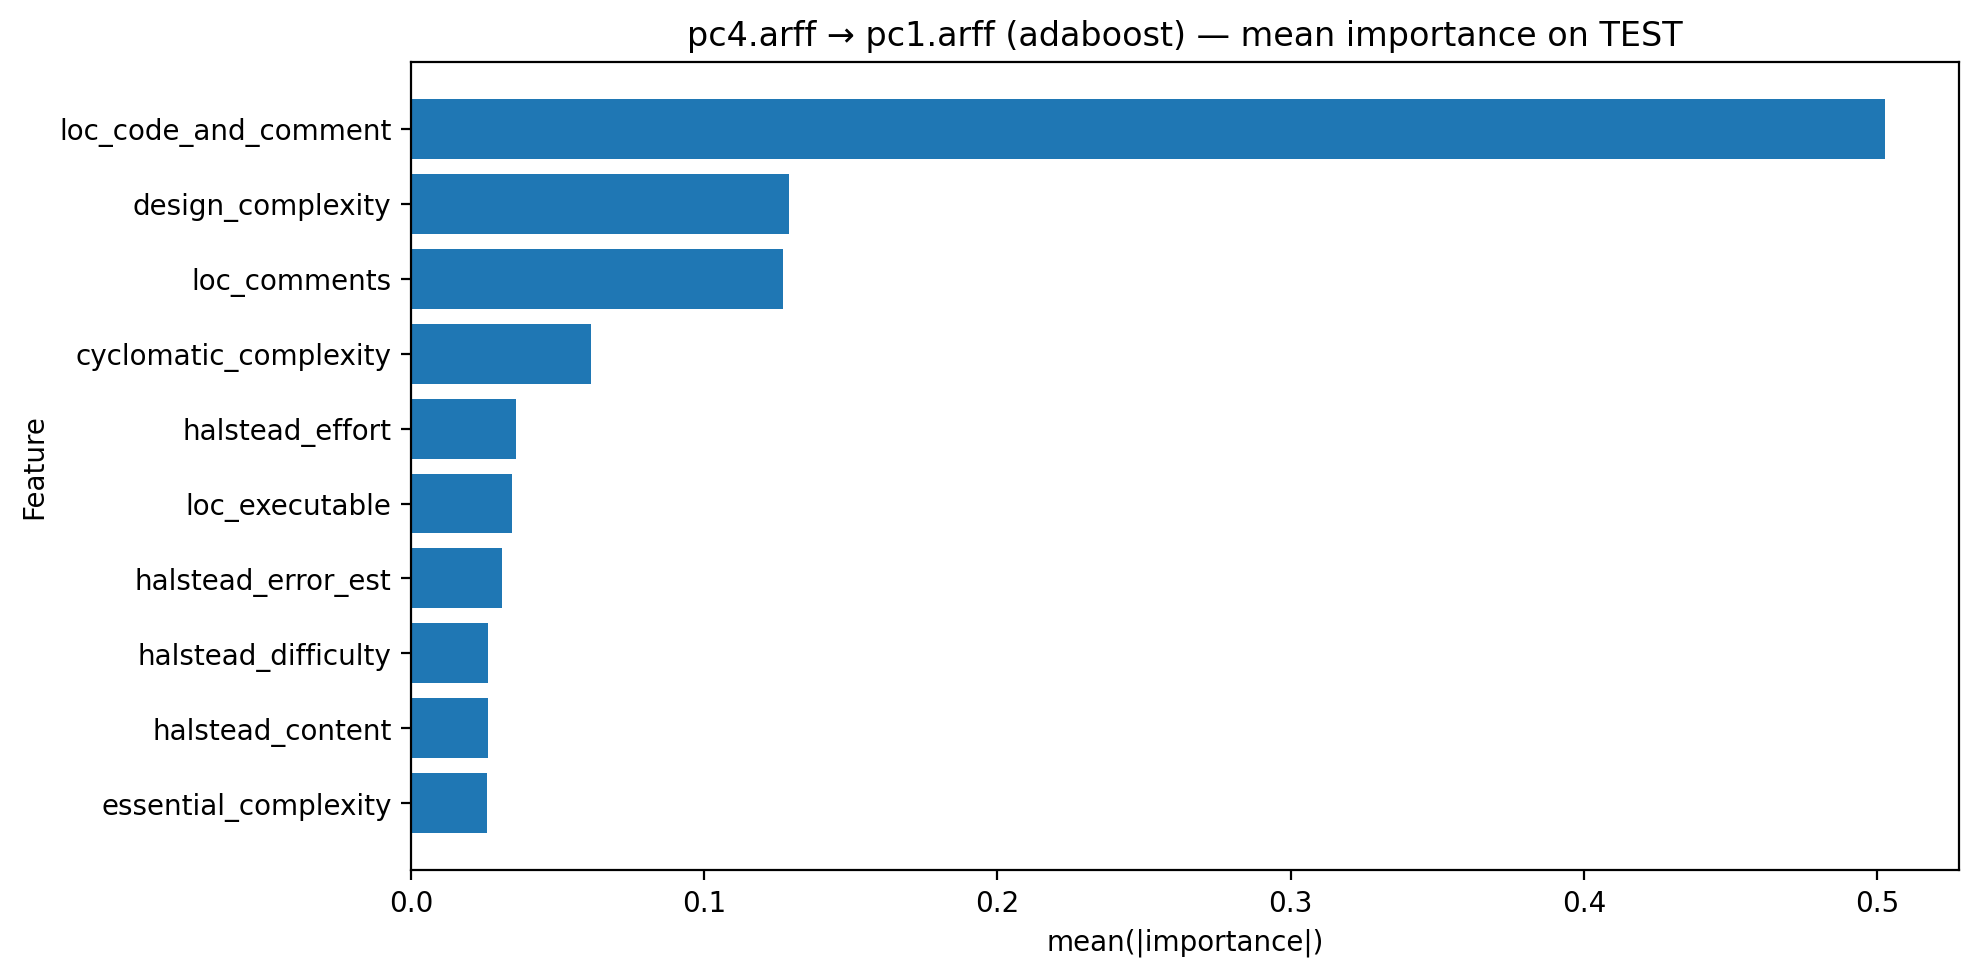
\includegraphics[width=\columnwidth]{top10_pc4_to_pc1_adaboost}
\caption{Top-10 influential metrics for \(\text{PC4}\rightarrow\text{PC1}\) (AdaBoost), based on mean test-set importance in the proposed pipeline.}
\label{fig:top10_pc4_pc1_adaboost}
\end{figure}

Proposed reliability distributions are summarized in Table~\ref{tab:reliability_dist}. Calibration quality is comparatively stable (ECE mean \(=0.0809\), std \(=0.0327\)), while GLR shows higher spread across model-transfer cases (std \(=0.1591\), range \([-0.2863, 0.5663]\)). Reconstructed Hit@k is near-saturated across pair-model means. This supports joint reporting of calibration and explanation-alignment metrics.

\begin{table}[t]
\caption{Distribution of Proposed Reliability/Calibration Metrics (96 Pair-Model Means)}
\label{tab:reliability_dist}
\centering
\footnotesize
\setlength{\tabcolsep}{4.0pt}
\renewcommand{\arraystretch}{1.10}
\begin{tabular}{|l|c|c|c|c|}
\hline
\textbf{Metric} & \textbf{Mean} & \textbf{Std} & \textbf{Min} & \textbf{Max} \\
\hline
Brier & 0.0824 & 0.0416 & 0.0051 & 0.1600 \\
\hline
ECE & 0.0809 & 0.0327 & 0.0100 & 0.1863 \\
\hline
GLR & 0.1627 & 0.1591 & -0.2863 & 0.5663 \\
\hline
Hit@k & 0.9998 & 0.0008 & 0.9950 & 1.0000 \\
\hline
ReliabilityScore & 0.8334 & 0.0267 & 0.7527 & 0.8946 \\
\hline
\end{tabular}
\renewcommand{\arraystretch}{1.0}
\normalsize
\end{table}

\subsection{Statistical Significance Analysis}
Paired WSR results on cross-project fold-matched values are summarized in Table~\ref{tab:wsr_cross_summary}. After excluding aggregate \texttt{MEAN} rows, each metric has 96 model-transfer tests.

Among predictive metrics, precision has the highest significant-improvement frequency (59/96, 61.5\%), while recall improves less often (21/96, 21.9\%). For reliability mappings, Concordance\(\rightarrow\)Hit@k is significant in 92/96 cases, Stability\(\rightarrow\)ECE is significant in all 96/96 cases after direction normalization (lower ECE treated as better), and Generalizability\(\rightarrow\)GLR shows no significant positive shifts.

\begin{table}[t]
\caption{Pair-Level WSR Summary Across 96 Model-Transfer Tests per Metric}
\label{tab:wsr_cross_summary}
\centering
\footnotesize
\setlength{\tabcolsep}{3.7pt}
\renewcommand{\arraystretch}{1.10}
\begin{tabular}{|l|c|c|c|c|}
\hline
\textbf{Metric} & \textbf{Sig@0.05} & \textbf{Rate} & \textbf{Mean Improvement} & \textbf{Median \(r\)} \\
\hline
AUC & 33/96 & 34.4\% & -0.0228 & -1.0 \\
\hline
F1 & 35/96 & 36.5\% & -0.0284 & -1.0 \\
\hline
Precision & 59/96 & 61.5\% & +0.0054 & +1.0 \\
\hline
Recall & 21/96 & 21.9\% & -0.1732 & -1.0 \\
\hline
Gen.\(\rightarrow\)GLR & 0/96 & 0.0\% & -0.6913 & -1.0 \\
\hline
Con.\(\rightarrow\)Hit@k & 92/96 & 95.8\% & +0.5028 & +1.0 \\
\hline
Stab.\(\rightarrow\)ECE & 96/96 & 100\% & +0.8107 & +1.0 \\
\hline
RI\(\rightarrow\)RS & 28/96 & 29.2\% & -0.0404 & -1.0 \\
\hline
\end{tabular}
\renewcommand{\arraystretch}{1.0}
\normalsize
\end{table}

The frequent median effect size magnitude \(|r|=1\) is expected for \(N=5\) paired folds when signed-rank direction is consistent. Together with Table~\ref{tab:overall_cross}, WSR outcomes confirm that the proposed pipeline primarily delivers a precision- and calibration-oriented shift, not a universal gain in all discrimination metrics.

\section{Threats to Validity}
\textbf{Internal validity:} Although preprocessing, feature alignment, and SMOTE are restricted to source-side training splits, implementation choices can still influence outcomes. In particular, threshold tuning and calibration settings may interact with class prevalence, and model-specific defaults in baseline notebooks may differ slightly from proposed scripts. We mitigated this risk by keeping a common directed-transfer protocol, storing fold-wise outputs, and matching baseline/proposed comparisons by model, pair, and fold index.

\textbf{Construct validity:} Reliability mappings compare non-identical constructs (Generalizability\(\leftrightarrow\)GLR, Stability\(\leftrightarrow\)ECE, and ReliabilityIndex\(\leftrightarrow\)ReliabilityScore). Therefore, direct magnitude comparison of mapped metrics is limited; interpretation should emphasize directionality and statistical significance rather than absolute equivalence. In addition, Hit@k contributes to ReliabilityScore but is not exported as a standalone fold-level column in the cross-project file, which limits metric-by-metric external reanalysis from one file alone.

\textbf{Conclusion validity:} Each model-transfer tuple uses \(N=5\) paired folds for WSR testing, which is standard but small, and can produce discrete \(p\)-value patterns and frequent extreme median effect sizes (e.g., \(|r|=1\)). We reduce over-interpretation by reporting both effect size and significance counts across all 96 transfer cases per metric.

\textbf{External validity:} Findings are derived from PROMISE PC1--PC4 and may not directly generalize to other repositories, languages, process models, or temporal release settings. Transfer direction effects observed here (especially when PC2 is source) may change under different feature spaces, defect definitions, or domain adaptation methods. Broader multi-repository and temporal-split evaluations are needed before claiming universal behavior.

\section{Conclusion and Future Work}
This work presented a reliability-aware XAI framework for cross-project defect prediction and evaluated it on PROMISE PC1--PC4 using 8 classifiers, 12 directed transfer pairs, and 96 model-transfer cases (3360 fold-level points per setting). The proposed pipeline (train-only SMOTE, calibration, threshold tuning, GLR/Hit@k/ECE-based reliability) changed the decision behavior in a measurable way. Relative to baseline, mean precision increased from 0.1924 to 0.1978 (\(+0.0054\)), while recall decreased from 0.3566 to 0.1834 (\(-0.1732\)); mean AUC changed from 0.7443 to 0.7215 (\(-0.0228\)) and mean F1 from 0.1757 to 0.1472 (\(-0.0284\)).

Model- and transfer-level analysis showed that ExtraTrees remained the most robust by cross-project AUC (0.7713 proposed), while LightGBM achieved the highest proposed ReliabilityScore (0.8512). Transfer direction was critical: the easiest direction was PC4\(\rightarrow\)PC2 (AUC 0.8057), and the hardest was PC2\(\rightarrow\)PC4 (AUC 0.5518). WSR results further confirmed non-uniform effects: precision improved significantly in 59/96 tests, and the Stability\(\rightarrow\)ECE mapping was significant in 96/96 tests. Overall, these results show that reliability should be reported jointly with predictive metrics, because calibration and explanation behavior can improve even when discrimination metrics do not uniformly increase.

Future work will focus on:
\begin{itemize}
\item Improving the precision-recall tradeoff using cost-sensitive learning and transfer-aware threshold optimization.
\item Extending evaluation to additional projects and distribution-shift settings (including temporal splits) to test external validity.
\item Adding uncertainty-aware reliability analysis (e.g., confidence intervals and bootstrap-based stability for GLR/Hit@k/ECE).
\item Unifying notebook workflows into a single reproducible pipeline and extending cross-project statistical testing to include Concordance\(\leftrightarrow\)Hit@k in the same export path.
\end{itemize}

\section*{Acknowledgment}
The author gratefully acknowledges the guidance and support of the project supervisor and the Department of Computer Science and Engineering, National Institute of Technology Warangal, for providing the academic environment and infrastructure needed for this work. The author also acknowledges the maintainers of the PROMISE software defect datasets and the open-source machine learning ecosystem used for experimentation and analysis.

\begin{thebibliography}{00}
\bibitem{r1} M. Begum, M. H. Shuvo, I. Ashraf, A. Al Mamun, J. Uddin, and M. A. Samad, ``Software defects identification: Results using machine learning and explainable artificial intelligence techniques,'' \emph{IEEE Access}, vol. 11, 2023.
\bibitem{r2} M. Begum, M. H. Shuvo, M. K. Nasir, A. Hossain, M. J. Hossain, I. Ashraf, J. Uddin, and M. A. Samad, ``LCNN: Lightweight CNN architecture for software defect feature identification using explainable AI,'' \emph{IEEE Access}, vol. 12, 2024.
\bibitem{r3} S. Haldar and L. F. Capretz, ``Explainable software defect prediction from cross-company project metrics using machine learning,'' in \emph{Proc. 7th Int. Conf. Intelligent Computing and Control Systems (ICICCS)}, 2023, pp. 150--157.
\bibitem{r4} P. Manchala and M. Bisi, ``Diversity based imbalance learning approach for software fault prediction using machine learning models,'' \emph{Applied Soft Computing}, vol. 124, 2022, Art. no. 109069.
\bibitem{r5} F. Ketata, Z. Al Masry, S. Yacoub, and N. Zerhouni, ``A methodology for reliability analysis of explainable machine learning: Application to endocrinology diseases,'' \emph{IEEE Access}, vol. 12, 2024.
\bibitem{r6} R. He, Y. Li, and C. Sun, ``Understanding software defect prediction through eXplainable neural additive models,'' \emph{IEEE Access}, vol. 13, 2025.
\bibitem{r7} T. Zimmermann, N. Nagappan, H. Gall, E. Giger, and B. Murphy, ``Cross-project defect prediction: A large scale experiment on data vs. domain vs. process,'' in \emph{Proc. 7th Joint Meeting ESEC/FSE}, 2009, pp. 91--100.
\bibitem{r8} B. Turhan, T. Menzies, A. Bener, and J. Di Stefano, ``On the relative value of cross-company and within-company data for defect prediction,'' in \emph{Proc. Int. Symp. Empirical Software Engineering and Measurement (ESEM)}, 2009, pp. 254--263.
\bibitem{r9} N. V. Chawla, K. W. Bowyer, L. O. Hall, and W. P. Kegelmeyer, ``SMOTE: Synthetic minority over-sampling technique,'' \emph{J. Artif. Intell. Res.}, vol. 16, pp. 321--357, 2002.
\bibitem{r10} M. T. Ribeiro, S. Singh, and C. Guestrin, ``Why should I trust you?: Explaining the predictions of any classifier,'' in \emph{Proc. 22nd ACM SIGKDD Int. Conf. Knowledge Discovery and Data Mining}, 2016, pp. 1135--1144.
\bibitem{r11} S. M. Lundberg and S.-I. Lee, ``A unified approach to interpreting model predictions,'' in \emph{Advances in Neural Information Processing Systems}, 2017, pp. 4765--4774.
\bibitem{r12} G. W. Brier, ``Verification of forecasts expressed in terms of probability,'' \emph{Monthly Weather Review}, vol. 78, no. 1, pp. 1--3, 1950.
\bibitem{r13} C. Guo, G. Pleiss, Y. Sun, and K. Q. Weinberger, ``On calibration of modern neural networks,'' in \emph{Proc. 34th Int. Conf. Machine Learning (ICML)}, 2017, pp. 1321--1330.
\bibitem{r14} M. P. Naeini, G. Cooper, and M. Hauskrecht, ``Obtaining well calibrated probabilities using Bayesian binning,'' in \emph{Proc. AAAI Conf. Artificial Intelligence}, 2015, pp. 2901--2907.
\bibitem{r15} J. Dem\v{s}ar, ``Statistical comparisons of classifiers over multiple data sets,'' \emph{J. Mach. Learn. Res.}, vol. 7, pp. 1--30, 2006.
\bibitem{r16} S. J. Pan and Q. Yang, ``A survey on transfer learning,'' \emph{IEEE Trans. Knowl. Data Eng.}, vol. 22, no. 10, pp. 1345--1359, 2010.
\end{thebibliography}

\end{document}
